% % % % % % % % % % % % % % % % % % % % % % % % % % % % % % % % % % % % % % % % % % % %
%                                                                                     %
% Short Sectioned Assignment LaTeX Template Version 1.0 (5/5/12)                      %
% This template has been downloaded from: http://www.LaTeXTemplates.com               %
%                                                                                     %
% Original author:  Frits Wenneker (http://www.howtotex.com)                          %
%                                                                                     %
% Modified by: Fco Javier Sueza Rodríguez (fcosueza@disroot.org)                      %
%                                                                                     %
% Changes:                                                                            %
%	    - Custom Chapters, Sections and Subsections (titlesec package)                %
%           - Document type scrbook (oneside)                                         %
%           - Use babel-lang-spanish package and marvosym                             %
%           - Use hyperref, enumitem, tcolorbox and glossaries packages               %
%           - Use Time New Roman (mathptmx), Helvetic and Courier fonts               %
%                                                                                     %
% License: CC BY-NC-SA 3.0 (http://creativecommons.org/licenses/by-nc-sa/3.0/)        %
%                                                                                     %
% % % % % % % % % % % % % % % % % % % % % % % % % % % % % % % % % % % % % % % % % % % %

%-----------------------------------------------%
%	              Packages                  %
%-----------------------------------------------%

\documentclass[paper=a4, fontsize=11pt, oneside]{scrbook}

% ---- Text Input/Output ----- %

\usepackage[T1]{fontenc}
\usepackage[utf8]{inputenc}
\usepackage{mathptmx}
\usepackage[scaled=.92]{helvet}
\usepackage{courier}
\usepackage[indent=12pt]{parskip}

\usepackage{geometry}
\geometry{verbose,tmargin=3cm,bmargin=3cm,lmargin=2.6cm,rmargin=2.6cm}

% ---- Language ----- %

\usepackage[spanish]{babel}
\usepackage{marvosym}

% ---- Another packages ---- %

\usepackage{amsmath,amsfonts,amsthm}
\usepackage{graphics,graphicx}
\usepackage{titlesec}
\usepackage{fancyhdr}
\usepackage{tcolorbox}
\usepackage{hyperref}
\usepackage{enumitem}
\usepackage[automake]{glossaries}

%--------------------------------------------------------------------%
%                      Customizing Document                          %
%--------------------------------------------------------------------%


% ----------- Custom Chapters, Sections and Subsections -------------- %

\titleformat{\chapter}[display]
			{\bfseries\Huge}
			{Tema \ \thechapter} {0.5ex}
			{\vspace{1ex}\centering}

\titleformat{\section}[hang]
			{\bfseries\Large}
			{\thesection}{0.5em}{}

\titleformat{\subsection}[hang]
			{\bfseries\large}
			{\thesubsection}{0.5em}{}

\titleformat{\subsubsection}[hang]
			{\bfseries\large}
			{\thesubsubsection}{0.5em}{}

\hypersetup{
    colorlinks=true,
    linkcolor=black,
    urlcolor=magenta
}

% ------------------- Custom heaaders and footers ------------------- %

\pagestyle{fancyplain}

\fancyhead[]{}
\fancyfoot[L]{}
\fancyfoot[C]{}
\fancyfoot[R]{\thepage}

\renewcommand{\headrulewidth}{0pt} % Remove header underlines
\renewcommand{\footrulewidth}{0pt} % Remove footer underlines

\setlength{\headheight}{13.6pt} % Customize the height of the header

% --------- Numbering equations, figures and tables ----------------- %

\numberwithin{equation}{section} % Number equations within sections
\numberwithin{figure}{section} % Number figures within sections
\numberwithin{table}{section} % Number tables within sections

% ------------------------ New Commands ----------------------------- %

\newcommand{\horrule}[1]{\rule{\linewidth}{#1}} % Create horizontal rule command


%----------------------------------------------------------------------------------------
%	TÍTULO Y DATOS DEL ALUMNO
%----------------------------------------------------------------------------------------

\title{
\vspace{10ex}
\normalfont \normalsize
\Huge \textbf{Tarea 9: Administración de Redes en Ubuntu 22.04 LTS}
}
\author{Francisco Javier Sueza Rodríguez}
\date{\normalsize\today}

%----------------------------------------------------------------------------------------
%                                     DOCUMENTO
%----------------------------------------------------------------------------------------
\begin{document}

\maketitle

\thispagestyle{empty}

\vspace{68ex}

\begin{center}
    \begin{tabular}{l l}
        \textbf{Centro}: & IES Aguadulce \\
        \textbf{Ciclo Formativo}: & Desarrollo Aplicaciones Web (Distancia)\\
        \textbf{Asignatura}: & Sistemas Informáticos\\
        \textbf{Tema}: & Tema 9 -  Administración de Redes en Ubuntu 22.04 LTS\\
    \end{tabular}
\end{center}

\newpage

\tableofcontents

\newpage

\listoffigures

\newpage

\section{Caso Práctico}
La empresa recibe el encargo de configurar servicios de red. Para ello, Ada asigna el trabajo a Antonio y Juan. En principio, se establece que serán cuatro los servicios de red a configurar. Además, se deberá configurar el entorno de red de manera adecuada.

\section{Ejercicios}

\subsection{Actividad 1: Configuración del Entorno de Red en Ubuntu}

\subsubsection{Enunciado}
Configura la MV de Ubuntu para que tenga siempre la misma dirección IP. Es decir, vamos a configurar de forma estática su dirección IP. Se puede hacer mediante comandos o con la interfaz gráfica (GUI) de Ubuntu. Para realizar esta actividad se recomienda consultar el siguiente documento: \href{https://www.juntadeandalucia.es/educacion/gestionafp/datos/tareas/DAM/SI_951965/2022-23/DAM_SI_9_2022-23_Individual__725769/Configuracion_de_red_para_Ubuntu.pdf}{Configuración de red en Ubuntu} (pdf).

La dirección IP asignada tiene que pertenecer a la red a través de la cual se comunicarán la máquina anfitriona y la virtual. Comprobarás que todo está correcto con un ping desde la MV a la puerta de enlace por defecto de tu red, un ping desde la máquina anfitriona a la virtual y otro desde la virtual a la anfitriona.

Las \textbf{capturas} deben mostrar, al menos:

\begin{itemize}
    \item Configuración de red de la máquina virtual.
    \item Configuración de red del equipo anfitrión.
    \item Ping positivo desde la MV a la puerta de enlace por defecto de tu red desde una terminal de Ubuntu.
    \item Ping positivo desde la máquina anfitriona a la MV.
    \item Ping positivo desde la MV a la anfitriona.
\end{itemize}

\subsubsection{Solución}
En este primer ejercicio vamos a asignar una \textbf{IP statica} a la interfaz ethernet de la Máquina Virtual. Ya que el sistema es una Ubuntu 22.04, debemos usar \textbf{Netplan}, la herramienta que usa actualmente Ubuntu y que sustituye a las net-tools tradicionales. Personalmente hubiera preferido usar el método tradicional, ya que es más genérico y puede usarse en cualquier distribución, pero como estamos estudiando Ubuntu, usaremos las herramientas que ésta incluye.

\textbf{Netplan} es una abstracción para un conjunto de aplicaciones que nos ayudan a configurar y obtener información de nuestra red y nuestros dispositivos de red, usa ficheros de configuración con formato \textbf{YAML} y funciona conjuntamente con \textbf{systemd-network}.

Para establecer la dirección ip estática de la interfaz de red, debemos editar el fichero \textbf{/etc/netplan/01-network-manager-all.yaml}, que es donde reside la configuración de red administrada por esta herramienta. Antes de eso podemos recopilar la información que necesitaremos con el comando \textbf{ip}, así sabremos la dirección actual de la interfaz de red, la subred a la que pertenece, dirección de broadcast, etc..

Una vez que sabemos esa información, usando nuestro editor preferido (nano, emacs, vi..) abrimos el fichero mencionado, teniendo en cuenta que debemos tener privilegios de root, por lo que incluiremos el comando \textbf{sudo} delante del editor que vayamos a usar, en nuestro caso el comando quedaría así:

\begin{figure}[H]
    \begin{tcolorbox}[sharp corners, colback=yellow!30, colframe=white!20]
        \scriptsize
        \begin{verbatim}
                sudo vi /etc/netplan/01-network-manager-all.yaml\end{verbatim}
    \end{tcolorbox}
\end{figure}


Si queremos, como precaución, podemos hacer una \textbf{copia de seguridad del fichero} de configuración, simplemente usando el comando \textbf{cp}, por si tocamos algo que no debemos que podamos restaurarlo sin problema.

Una vez abierto el fichero, vamos a introducir los\textbf{ datos de nuestra configuración de red}, los cuales podemos ver en la siguiente captura con más detalle.

\begin{figure}[H]
    \centering
    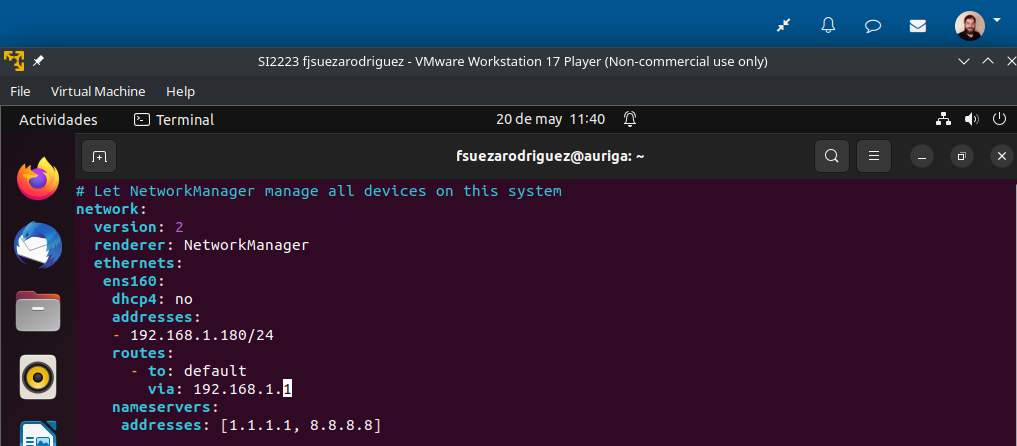
\includegraphics[scale=0.50]{netconfig-1.png}
    \caption{Configuración ip estática con Netplan}
\end{figure}

Solo un par de \textbf{comentarios} sobre la configuración que hemos puesto. La opción \textbf{gateway4} para indicar la puerta de enlace esta ya obsoleta, por lo que hemos tenido que usar \textbf{routes} con la opción \textbf{default} para indicar la puerta de enlace hacia internet. Además, hemos aprovechado para cambiar el \textbf{servidores DNS} y que nuestra interfaz use los proporcionados por \textbf{Cloudfare}, los cuales suelen ser bastante rápidos.

Tras guardar el fichero de configuración, hemos usado el comando \textbf{netplan try} para ver si la configuración es correcta, como ha sido nuestro caso.

Para comprobar que la configuración de red se ha \textbf{realizado correctamente}, hemos llevado a cabo los siguientes pasos:

\begin{enumerate}
    \item En primer lugar hemos \textbf{reiniciado} la máquina virtual, para comprobar que al reiniciarla la configuración de red es persistente, y se mantiene la dirección IP estática que le habíamos asignado.

    \item A continuación, hemos usado el comando \textbf{ip a} tanto en la \textbf{máquina virtual} como en el \textbf{SO operativo host}, que también es una Ubuntu 22.04 LTS. El resultado de ambos comandos los podemos ver en la siguientes capturas de pantalla.

    \begin{figure}[H]
        \centering
        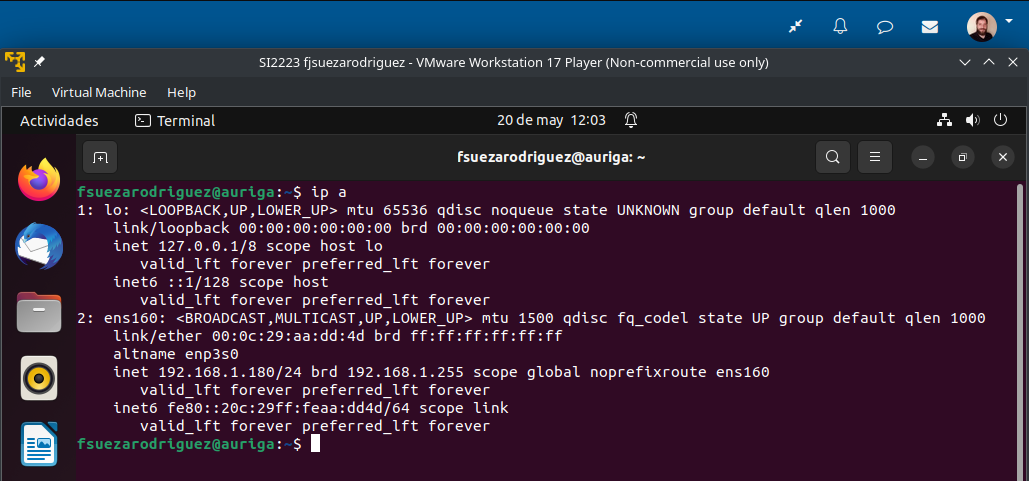
\includegraphics[scale=0.45]{netconfig-2.png}
        \caption{Configuración de red en la máquina virtual}
    \end{figure}

    \begin{figure}[H]
        \centering
        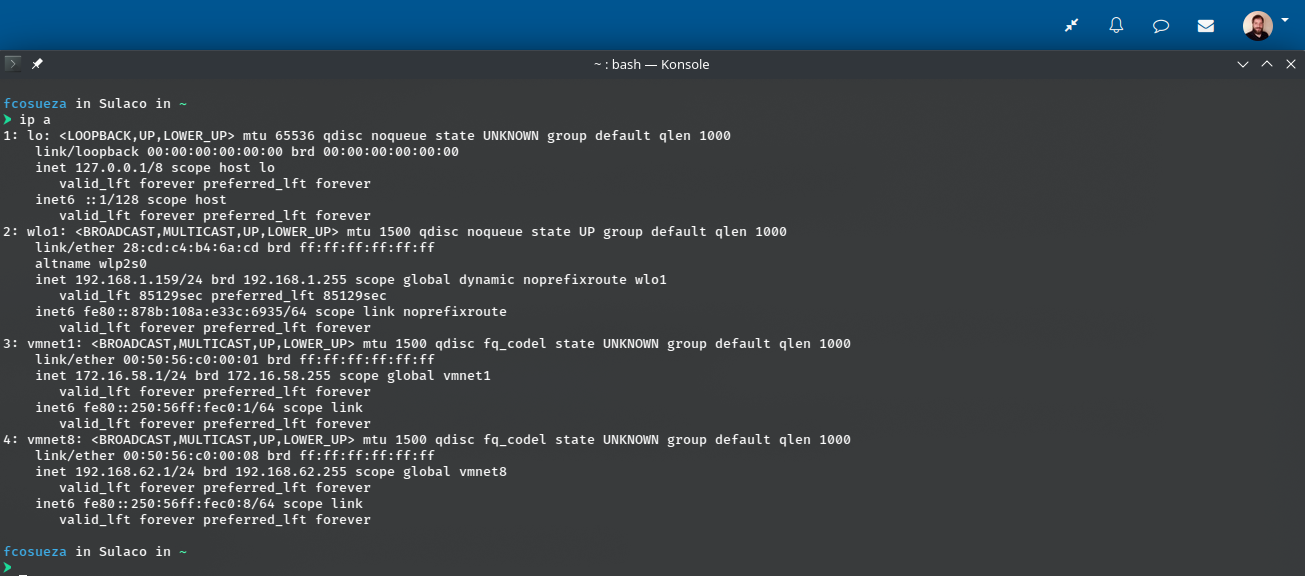
\includegraphics[scale=0.35]{netconfig-3.png}
        \caption{Configuración de red en el SO hots}
    \end{figure}

    Como vemos en la figura 2.2, la configuración de red de nuestra máquina virtual está correctamente.

    \item El siguiente paso será hacer \textbf{ping} a diferentes destinos desde la máquina virtual para comprobar que la conexión funciona correctamente. Los ping que hemos realizado son los siguientes:

    \begin{itemize}
        \item \textbf{Desde la MV a la puerta de enlace}:
        \begin{figure}[H]
            \centering
            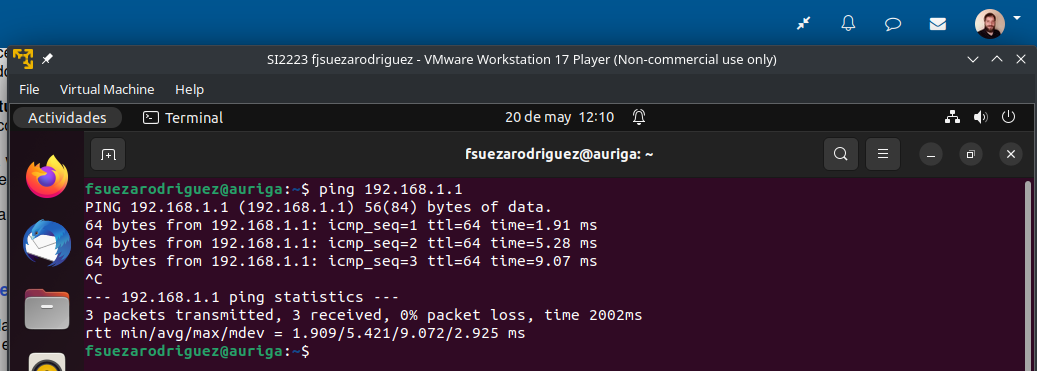
\includegraphics[scale=0.42]{ping-1.png}
            \caption{Ping desde la MV a la puerta de enlace}
        \end{figure}

        \item \textbf{Desde la máquina anfitriona a la MV}:
        \begin{figure}[H]
            \centering
            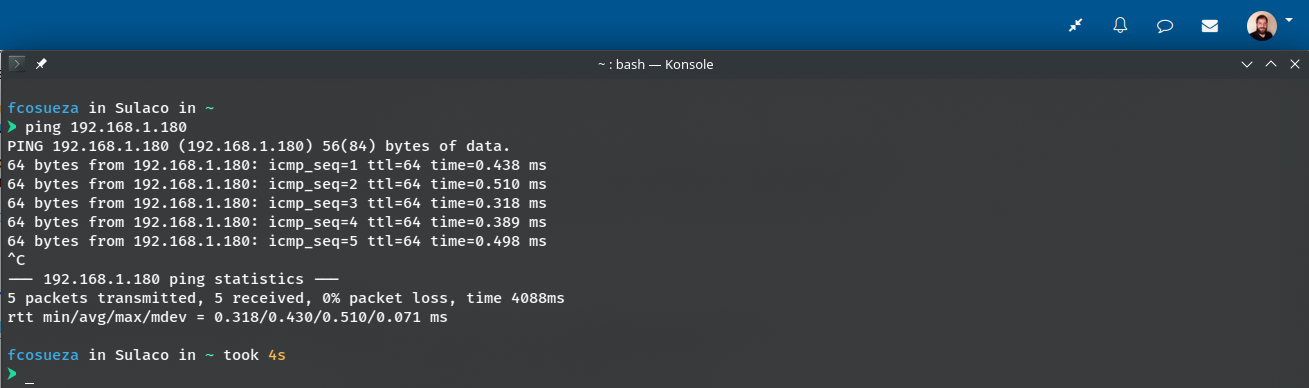
\includegraphics[scale=0.38]{ping-2.png}
            \caption{Ping desde máquina anfitriona a la MV}
        \end{figure}

        \item \textbf{Desde la MV a la máquina anfitriona}:
        \begin{figure}[H]
            \centering
            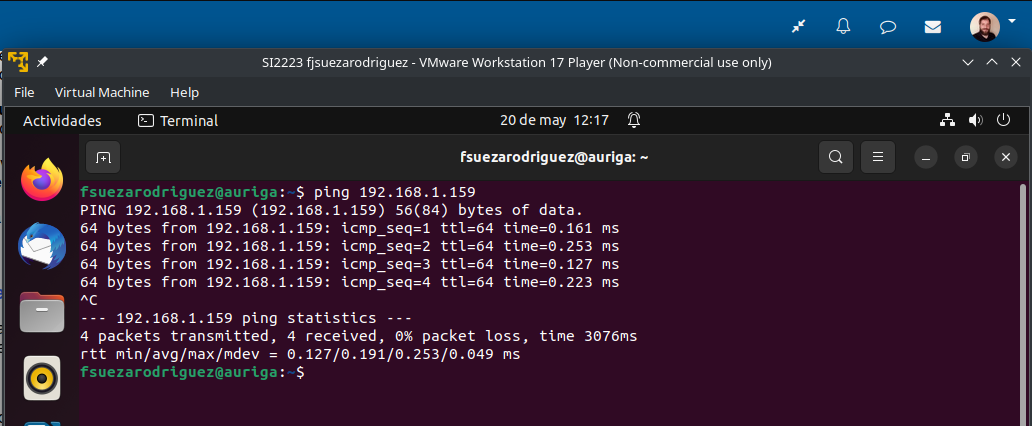
\includegraphics[scale=0.45]{ping-3.png}
            \caption{Ping desde la MV a la máquina anfitriona}
        \end{figure}
    \end{itemize}
\end{enumerate}

Como podemos comprobar, todas las conexiones funcionan correctamente en ambos sentidos. Aunque no se incluye aquí la captura, también se ha realizado ping a servidores externos a la red local desde la MV para comprobar que hay conexión a internet correctamente, siendo los resultados positivos.

\subsection{Actividad 2: Correo y Búsqueda de Información}

\subsubsection{Enunciado}
Desde la MV, haz login en el aula virtual de Sistemas Informáticos y envía a tu profesor un correo a través de la plataforma (icono del ``sobre'' a la izquierda de tu foto de perfil de usuario). El correo tendrá como asunto ``<Tu\_Nombre> Tarea 9.- Documentación de Ubuntu 22.04'', y en el cuerpo del asunto habrá un breve texto a tu elección, y se incluirá un enlace a la página oficial de documentación de Ubuntu Desktop 22.04.

Las \textbf{capturas} deben mostrar, al menos:
\begin{itemize}
    \item La página oficial de documentación de Ubuntu Desktop 22.04.
    \item El correo que se envía a través de la plataforma desde la MV redactado.
\end{itemize}

\subsubsection{Solución}
En primer lugar, hemos buscado un artículo en al documentación oficial de Ubuntu, el concreto el artículo \textbf{About Gnome}, el cual podemos ver en la siguiente captura.

\begin{figure}[H]
    \centering
    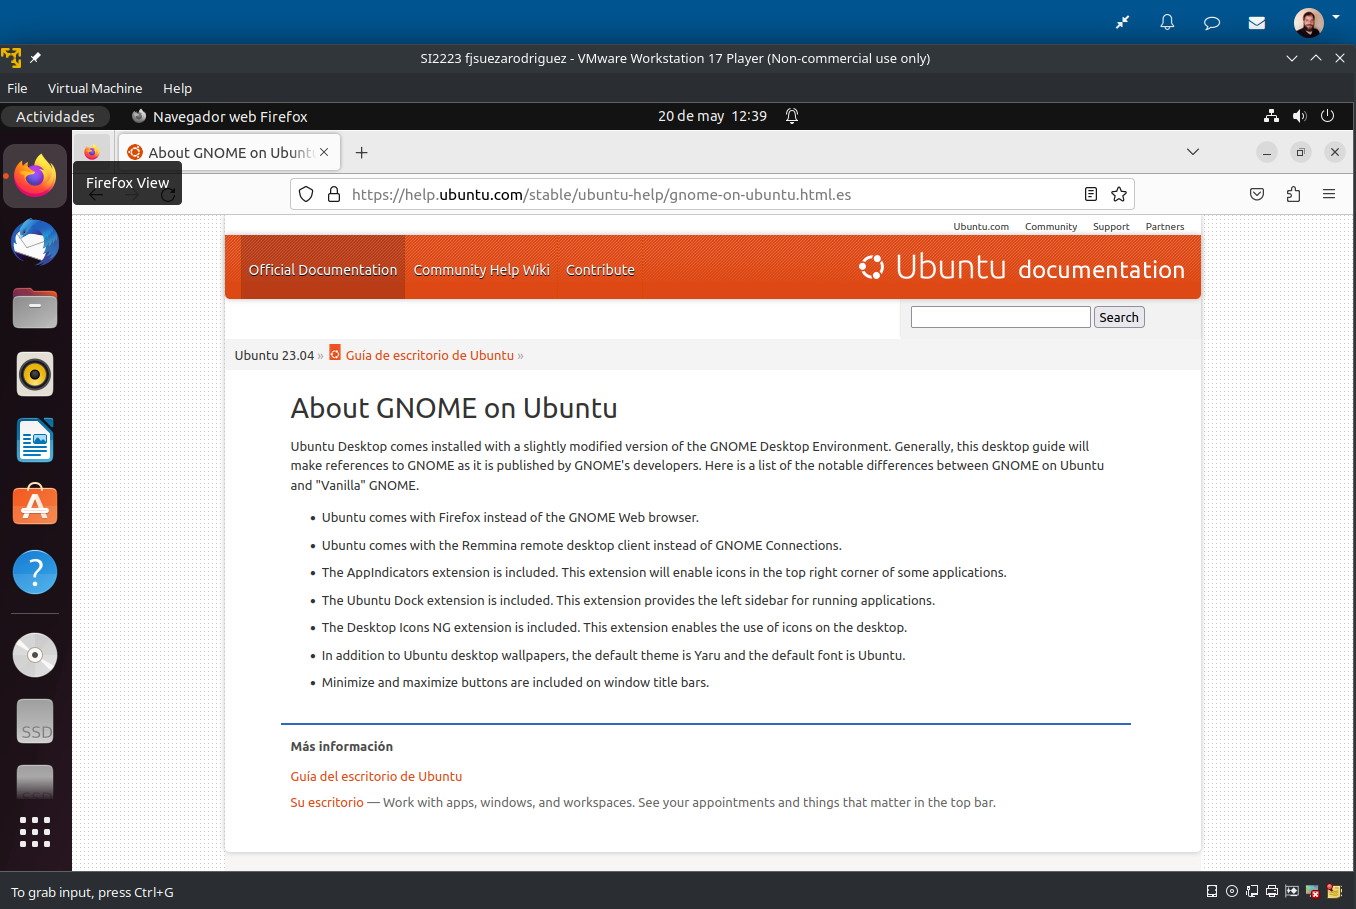
\includegraphics[scale=0.37]{ubuntuDoc.png}
    \caption{Artículo documentación oficial Ubuntu}
\end{figure}

A continuación, hemos \textbf{conectado a la plataforma} y \textbf{redactado el mensaje} al profesor con los datos que se especifican en el enunciado, como vemos a continuación.

\begin{figure}[H]
    \centering
    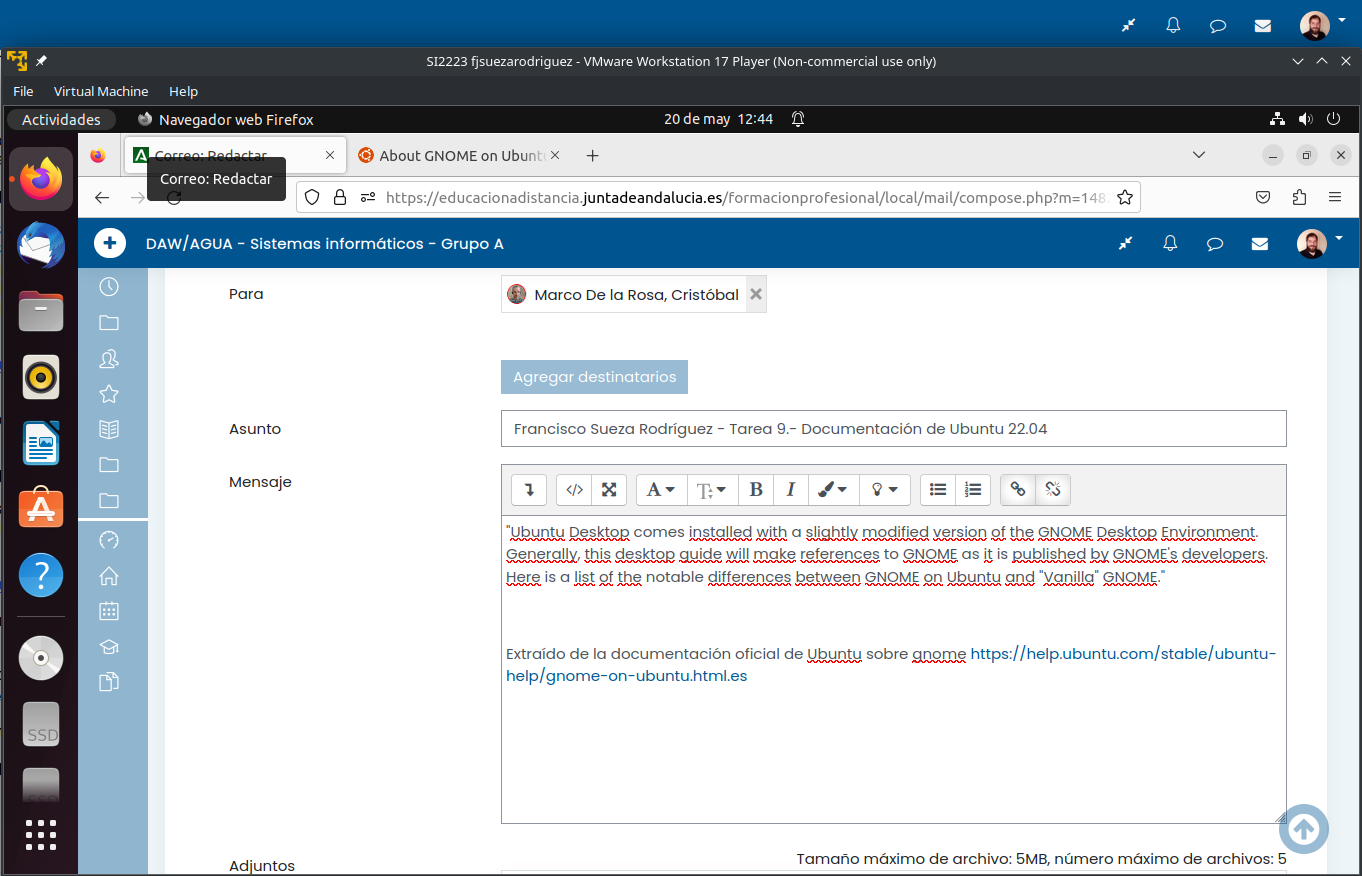
\includegraphics[scale=0.37]{emailProf.png}
    \caption{Correo desde la plataforma al profesor}
\end{figure}

\subsection{Actividad 3: Compartir recursos en la red}

\subsubsection{Enunciado}
Crea en tu máquina anfitriona una carpeta y compártela en red. A continuación, accede a dicha carpeta desde la máquina virtual Ubuntu y crea un fichero de texto nuevo en su interior con tu nombre. \textbf{Se debe hacer a través de la red local} y en ningún caso usando la opción de carpetas compartidas que ofrezca el software de virtualización usado.

Esta operación suele ser muy simple y no debería requerir ninguna instalación, pero dependiendo de qué SO tengas en tu máquina anfitriona es posible que necesites instalar en ella o en la MV distintos paquetes (Samba, NFS, APFS, etc.).

Esquema de conexión: Máquina virtual con Ubuntu > Carpeta compartida en SO anfitrión.

Las \textbf{capturas} deben mostrar, al menos:

\begin{itemize}
    \item Creación y compartición de la carpeta en la máquina real.
    \item Acceso a ella desde la MV. Se debe ver y explicar claramente cómo se ha hecho el acceso.
    \item Creación y edición de un fichero de texto desde la MV.
\end{itemize}

\subsubsection{Solución}






% Bibliography

%\newpage
%\bibliography{citas}
%\bibliographystyle{unsrt}

\end{document}